%! TEX root = main.tex

\graphicspath{{00_Images/09_chapter/}}

\chapter{Thermionic Valves}
\label{ch:valves}

\section{Brief History and the Thermionic Diode}
\label{sc:91}

Before the invention of the transistor, every amplifying device relied on the thermionic valve, also called the vacuum tube, and these devices still survive today in high-end audio and in guitar amplification because of their distinctive overload behavior.
The story begins in 1880, when Thomas Edison observed a one-way current flowing across the vacuum gap of an incandescent lamp, an unexplained phenomenon that became known as the Edison effect.
The carrier responsible was identified as the electron by J. J. Thomson in 1897, and in 1904 J. A. Fleming exploited the effect to build the first two-electrode valve, the thermionic diode, which served as the rectifier of early radio receivers.
The decisive step for amplification came in 1906, when Lee de Forest inserted a third electrode, the grid, creating the triode and with it the first electronic amplifying device.
The operating principle of every valve is thermionic emission.
When a cathode is heated to roughly \SI{1050}{\kelvin}, a fraction of its conduction electrons acquires enough kinetic energy to overcome the surface potential barrier, set by the work function of the material, and escapes into the surrounding vacuum.
A positively biased anode, called the plate, then collects these electrons, establishing a space current that flows from cathode to plate through the evacuated envelope, the high vacuum being essential to prevent collisions with residual gas atoms.
The conduction is intrinsically unidirectional: if the plate is made negative with respect to the cathode the emitted electrons are repelled and no current flows, so the thermionic diode behaves as a rectifier.

\begin{figure}[!htb]
    \centering
    \subfloat[Diode geometry: a heated cathode emits electrons collected by a positive plate across the vacuum]{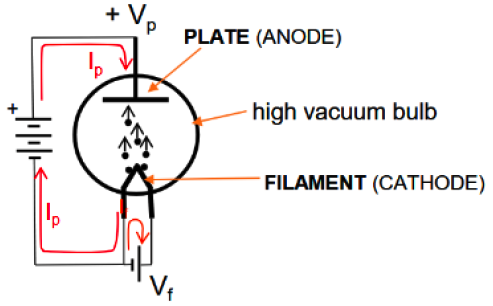
\includegraphics[height=0.20\textheight]{Diode.png}}
    \hfill
    \subfloat[Plate characteristic: space-charge-limited and emission-limited (saturation) regions]{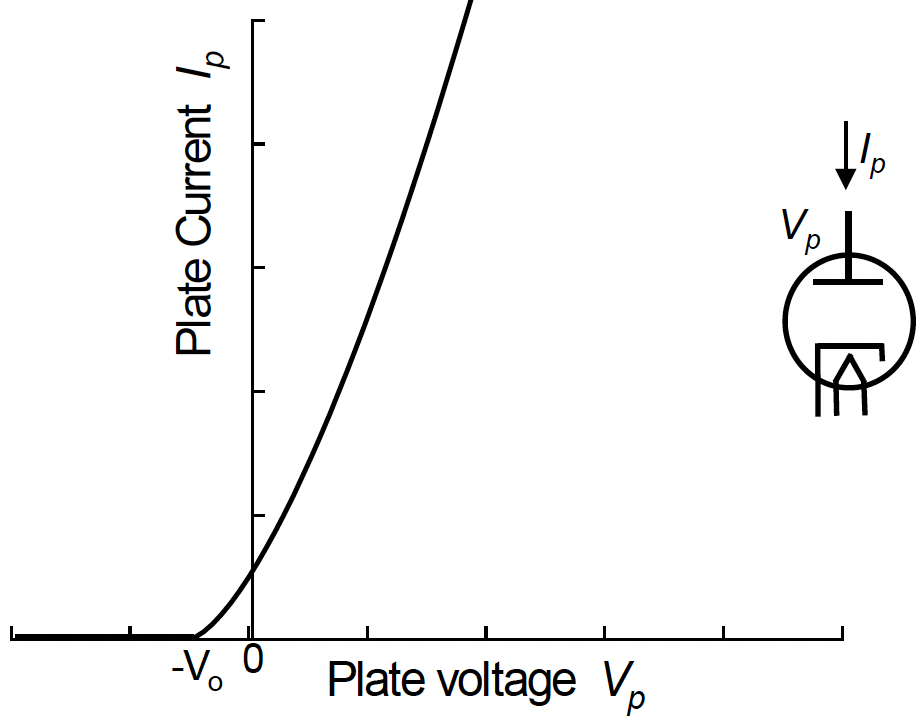
\includegraphics[height=0.20\textheight]{Diode_IV.png}}
    \caption{The thermionic diode and its current-voltage characteristic}
    \label{fig:thermionicDiode}
\end{figure}

The plate characteristic of figure \ref{fig:thermionicDiode} exhibits two regimes.
For moderate positive plate voltage the current is limited by the cloud of electrons hovering near the cathode, the space charge, and obeys the Child-Langmuir law
\[
I_p = K V_p^{3/2}
\]
At higher plate voltage every emitted electron is collected and the current saturates at the emission-limited value set by the Richardson-Dushman law
\[
I_s = S A^{*} T^2 e^{-q\phi / k_B T}
\]
where \(S\) is the cathode area, \(A^{*}\) the Richardson constant, \(T\) the absolute temperature, \(q\) the electron charge, \(k_B\) the Boltzmann constant, and \(\phi\) the work function of the cathode surface, a few electronvolts for typical emitter materials.

\section{Triodes and Small-Signal Parameters}
\label{sc:92}

The triode is obtained by interposing a control grid, a fine wire mesh, between cathode and plate.
Because the grid sits much closer to the cathode than the plate does, a small voltage applied to it exerts a strong electrostatic influence on the space current, far stronger than an equal change of plate voltage would.
The grid is normally held slightly negative with respect to the cathode, so it draws essentially no current, yet it modulates a large plate current: the triode is therefore the thermionic realization of a voltage-controlled current source, the same role played by the transistors of chapter \ref{ch:transistors}.

\begin{figure}[!htb]
    \centering
    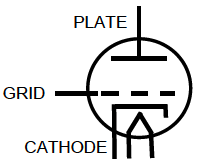
\includegraphics[width=0.40\textwidth]{triode.png}
    \caption{Schematic symbol of the triode, with cathode, control grid, and plate}
    \label{fig:triodeSymbol}
\end{figure}

The large-signal characteristic of the triode collects the grid and plate influence into a single controlling combination:
\[
I_p + I_g = K(\mu V_g + V_p)^m, \qquad I_g \approx 0
\]
so that the plate current depends on the weighted sum \(\mu V_g + V_p\), the factor \(\mu\) expressing how many times more effective the grid is than the plate in controlling the current.
This nonlinear law is linearized around a chosen operating point, defined by the bias values \(\bar V_g\), \(\bar V_p\), and \(\bar I_p\), exactly as done for transistors, yielding a small-signal model governed by three incremental parameters:
\[
r_p = \left.\frac{\partial V_p}{\partial I_p}\right|_{V_g = \bar V_g}, \qquad g_m = \left.\frac{\partial I_p}{\partial V_g}\right|_{V_p = \bar V_p}, \qquad \mu = \left.\frac{\partial V_p}{\partial V_g}\right|_{I_p = \bar I_p} = g_m r_p
\]
The plate resistance \(r_p\) is the output resistance seen at the plate, the transconductance \(g_m\) is the control of plate current by grid voltage, and the amplification factor \(\mu\) is their product, the maximum voltage gain the device can provide.
The triple \((\mu, g_m, r_p)\) completely characterizes the small-signal behavior of the valve near its operating point, and only two of the three are independent because of the relation \(\mu = g_m r_p\).

\begin{figure}[!htb]
    \centering
    \subfloat[Controlled current source \(g_m v_g\) in parallel with \(r_p\)]{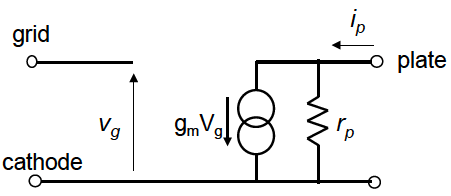
\includegraphics[height=0.14\textheight]{Triode_small_signal_circuit_1.png}}
    \hfill
    \subfloat[Equivalent voltage source \(\mu v_g\) in series with \(r_p\)]{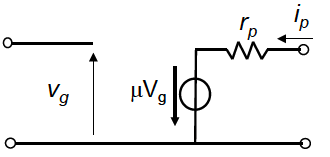
\includegraphics[height=0.14\textheight]{Triode_small_signal_circuit_2.png}}
    \caption{The two equivalent small-signal models of the triode: the transconductance form and the amplification-factor form}
    \label{fig:triodeSmallSignal}
\end{figure}

The two equivalent circuits of figure \ref{fig:triodeSmallSignal} are the valve counterparts of the Thevenin and Norton representations: a current source \(g_m v_g\) in parallel with \(r_p\), or a voltage source \(\mu v_g\) in series with \(r_p\).
In practice the three parameters are read directly from the datasheet plate-characteristic family, the curves of \(I_p\) against \(V_p\) drawn for a set of fixed grid voltages \(V_g\).
On the family of figure \ref{fig:triodeCurves} the local slope of a curve with respect to \(V_p\) yields the conductance \(1/r_p\), while the vertical spacing between adjacent curves, taken at fixed plate voltage, yields the transconductance \(g_m\) as the change of plate current per unit change of grid voltage.

\begin{figure}[!htb]
    \centering
    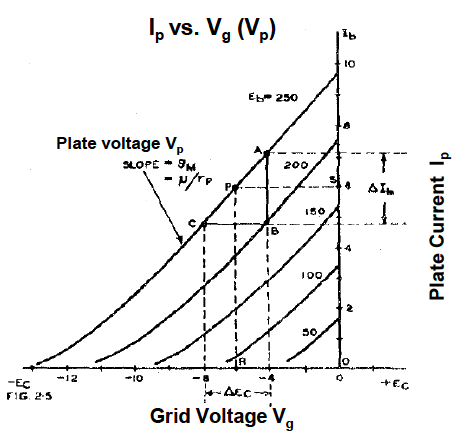
\includegraphics[width=0.40\textwidth]{Plate_mutual_characteristics.png}
    \caption{Plate-characteristic family of a triode: the slope along \(V_p\) gives \(1/r_p\), the spacing between iso-\(V_g\) curves gives \(g_m\), and their ratio gives \(\mu\)}
    \label{fig:triodeCurves}
\end{figure}

\section{Tetrodes and Pentodes}
\label{sc:93}

The triode suffers from a parasitic capacitance between the control grid and the plate.
At audio and radio frequencies this capacitance couples the output back to the input, an unwanted feedback aggravated by the Miller effect, which multiplies the apparent grid-to-plate capacitance by the stage gain and so limits the usable bandwidth.

\subsection{The Tetrode and Secondary Emission}
\label{ssc:931}

The tetrode addresses this problem by inserting a second grid \(g_2\), the screen grid, between the control grid \(g_1\) and the plate.
The screen is held at a fixed positive DC potential and is short-circuited to ground for AC by a bypass capacitor, so that it acts as an electrostatic shield: it breaks the direct line between control grid and plate and effectively cancels the grid-to-plate capacitance, suppressing the feedback and extending the bandwidth.

\begin{figure}[!htb]
    \centering
    \subfloat[Tetrode: the screen grid \(g_2\) shields \(g_1\) from the plate]{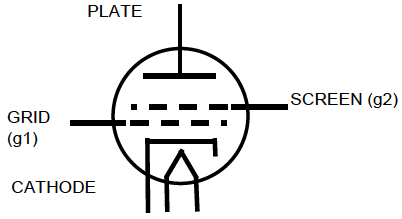
\includegraphics[height=0.16\textheight]{tetrode.png}}
    \hspace{1.5cm}
    \subfloat[Plate and screen currents against plate voltage, with the secondary-emission kink]{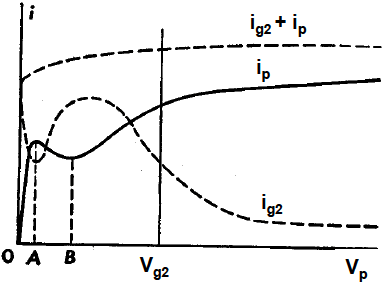
\includegraphics[height=0.16\textheight]{Tetrode_Ip_Vp.png}}
    \caption{The tetrode and its characteristic, distorted by secondary emission in the region where the plate voltage is below the screen voltage}
    \label{fig:tetrode}
\end{figure}

The screen, however, introduces a new defect known as secondary emission, visible as the kink of figure \ref{fig:tetrode}.
Electrons arriving at the plate with high energy dislodge further electrons from its surface, and when the plate voltage is lower than the screen voltage these secondary electrons are attracted to the screen rather than returning to the plate.
The result is a region in which the plate current actually decreases as the plate voltage rises, while the screen current increases by the same amount, an anomalous negative-resistance behavior that makes the tetrode unsuitable as a clean amplifier over part of its range.
Above the screen voltage the plate regains control of the secondary electrons and the current resumes its normal rise.

\subsection{The Pentode and the Flat Characteristic}
\label{ssc:932}

The pentode cures secondary emission by adding a third grid \(g_3\), the suppressor grid, placed between the screen and the plate and connected to the cathode potential.
Being negative with respect to the plate, the suppressor repels the low-energy secondary electrons back toward the plate that emitted them, eliminating the kink and restoring a smooth, monotonic characteristic.

\begin{figure}[!htb]
    \centering
    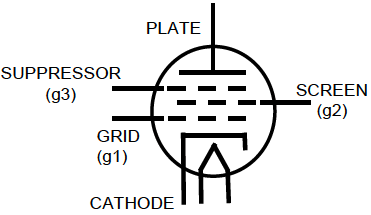
\includegraphics[width=0.40\textwidth]{pentode.png}
    \caption{The pentode: the suppressor grid \(g_3\), tied to the cathode, returns the secondary electrons to the plate}
    \label{fig:pentode}
\end{figure}

The decisive consequence is the shape of the plate characteristic.
Once the suppressor is in place the plate current becomes almost independent of the plate voltage above a low knee, so the curves run nearly flat and horizontal, in contrast with the steeply rising triode curves and the kinked tetrode curves.

\begin{figure}[!htb]
    \centering
    \subfloat[Triode versus pentode plate characteristics]{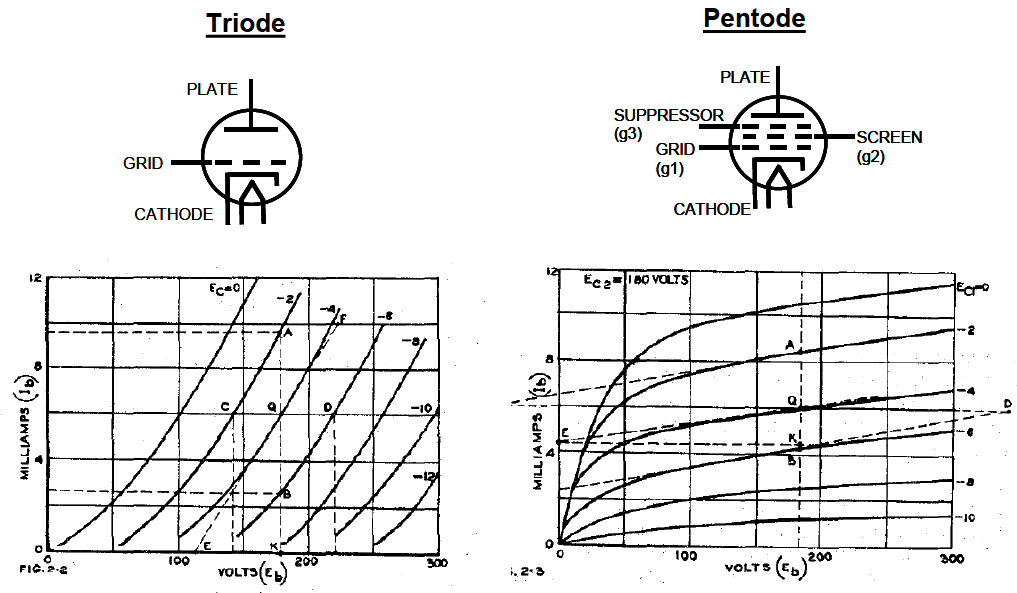
\includegraphics[height=0.17\textheight]{Triode_vs_Pentode.png}}
    \hfill
    \subfloat[Tetrode versus pentode plate characteristics]{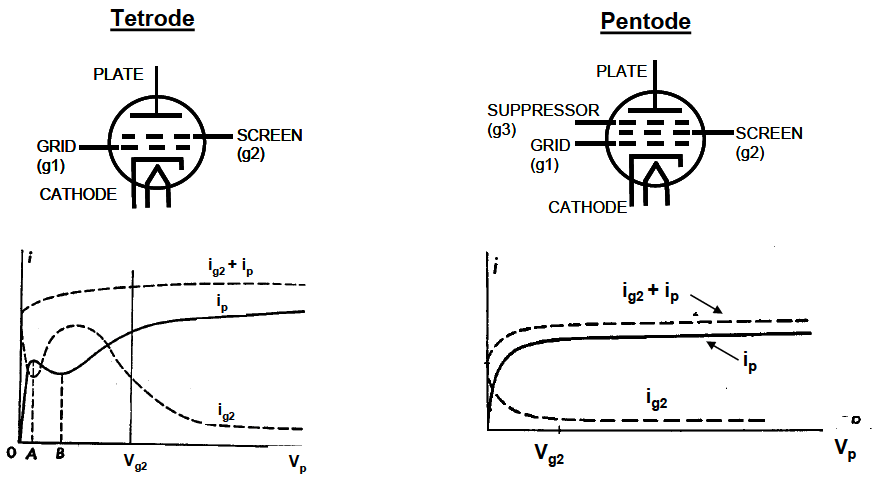
\includegraphics[height=0.17\textheight]{tetrode_vs_pentode.png}}
    \caption{Comparison of the three valve families: the pentode keeps the plate current nearly constant over a wide range of plate voltage}
    \label{fig:valveComparison}
\end{figure}

A flat plate characteristic means a very small slope along \(V_p\), and therefore a very high dynamic plate resistance \(r_p = \partial V_p / \partial I_p\).
Since the amplification factor is \(\mu = g_m r_p\), a high \(r_p\) at comparable transconductance gives the pentode a much larger effective amplification factor than the triode, as the comparison of figure \ref{fig:valveComparison} shows.
Just as importantly, the flatness allows the plate voltage to swing over a very wide range without the plate current, and hence the gain, collapsing.
This combination of high gain and large undistorted voltage swing is precisely what an output stage requires, which is why pentodes, and the closely related beam tetrodes, are the devices of choice for the power section of an amplifier, while triodes, with their lower \(r_p\), are preferred where linearity rather than raw gain is paramount.

\section{Application: Preamplifier and Power Stages}
\label{sc:94}

A complete valve guitar amplifier, such as the Fender Bassman taken as reference in the lectures, organizes these devices according to the task each stage must perform.
The low-level signal from the instrument is handled by triodes in the preamplifier, where linearity and controlled overdrive matter more than power, while the loudspeaker is driven by pentodes in the output stage, where large power delivery is the goal.

\subsection{The Two-Stage Triode Preamplifier}
\label{ssc:941}

The canonical preamplifier building block is a two-stage triode amplifier, in which the input is AC-coupled by a DC-blocking capacitor and the two stages perform complementary roles.

\begin{figure}[!htb]
    \centering
    \subfloat[Circuit schematic of the two-stage amplifier]{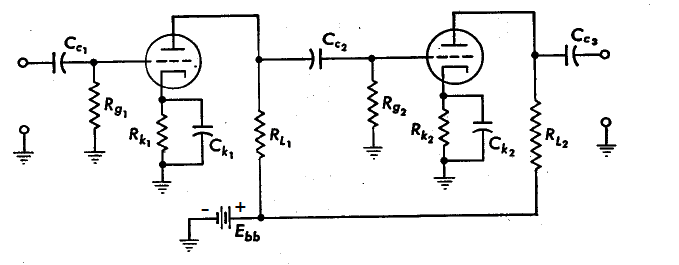
\includegraphics[height=0.22\textheight]{two_stage_triode_scheme.png}}
    \hfill
    \subfloat[Small-signal equivalent of the two stages]{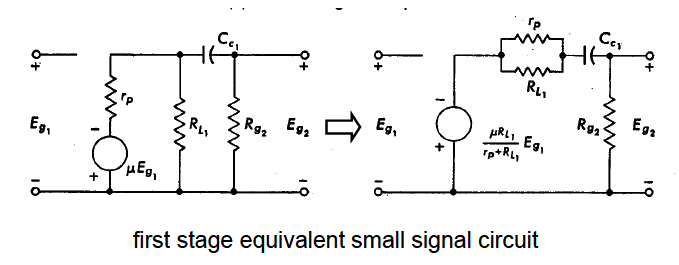
\includegraphics[height=0.22\textheight]{two_stage_triode_small_signal.png}}
    \caption{Two-stage triode preamplifier: a common-cathode voltage-gain stage followed by a cathode-follower buffer}
    \label{fig:twoStageTriode}
\end{figure}

The first stage is a common-cathode amplifier, the valve equivalent of the common-emitter stage, which provides voltage gain.
With a load resistance \(R_L\) at the plate, its small-signal output voltage is
\[
v_{out} = -g_m v_g (R_L || r_p) = -\mu v_g \frac{R_L}{R_L + r_p}
\]
the negative sign marking the phase inversion of a gain stage, and the gain approaching the full amplification factor \(\mu\) when the load dominates the plate resistance.
For a typical small-signal double triode such as the 12AU7A used in the worked example, the operating point yields \(g_m \approx \SI{700}{\micro\siemens}\), \(r_p \approx \SI{17}{\kilo\ohm}\), and therefore \(\mu = g_m r_p \approx 12\), a representative voltage gain for one preamplifier stage.

The second stage is a cathode follower, the valve counterpart of the emitter follower analyzed in section \ref{sc:74}.
It provides no voltage gain, with \(A_V \approx 1\), but presents a low output impedance of order
\[
Z_{out} \approx \frac{1}{g_m}
\]
so that it buffers the high-impedance gain stage and drives the following network, typically the passive tone stack, without loading it.
Preamplifier valves are commonly packaged as double triodes, two independent triodes in one envelope, such as the 12AX7, also designated ECC83, used in the preamplifier stages of the Marshall JCM 800 discussed in the case study of section \ref{sc:JCM800}.

\begin{figure}[!htb]
    \centering
    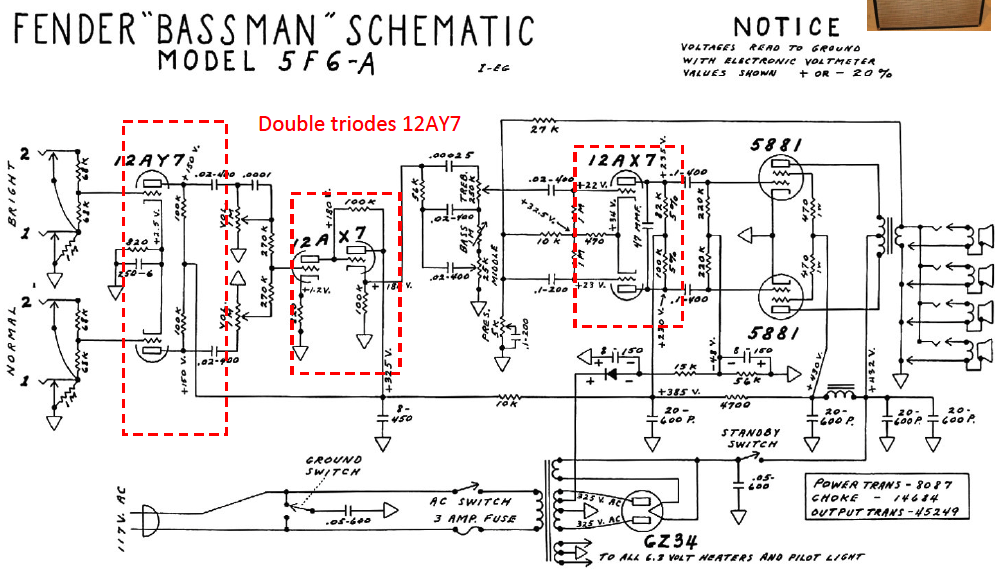
\includegraphics[width=0.78\textwidth]{Fender_Bassman_schematics_2.png}
    \caption{Preamplifier section of the Fender Bassman, with the double triodes arranged as cascaded common-cathode gain stages and cathode-follower buffers}
    \label{fig:bassman}
\end{figure}

\subsection{The Pentode Power Stage}
\label{ssc:942}

The output stage delivers the power required by the loudspeaker, and here the flat, high-\(r_p\) characteristic of the pentode is exploited to obtain a large voltage swing across the load while preserving gain.
Because a single device cannot supply the necessary current, several power pentodes are operated in parallel, their combined plate currents summed into the primary of an output transformer that matches the high plate impedance of the valves to the low impedance of the loudspeaker.

\begin{figure}[!htb]
    \centering
    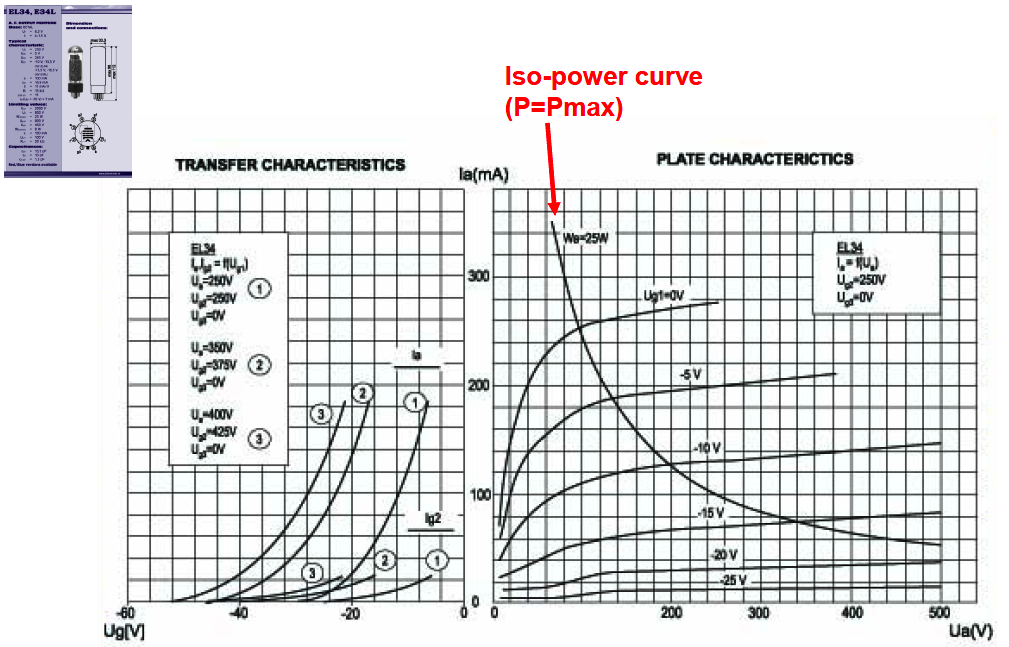
\includegraphics[width=0.55\textwidth]{EL34.png}
    \caption{Plate characteristics of the EL34 power pentode: the operating point is chosen below the iso-power dissipation limit to keep the device within its safe thermal range}
    \label{fig:el34}
\end{figure}

A representative power pentode is the EL34, whose plate characteristics appear in figure \ref{fig:el34}.
The operating point is always selected below the iso-power hyperbolas that mark the maximum allowable plate dissipation, ensuring that the product of plate voltage and plate current stays within the safe thermal limit of the device.
The detailed treatment of how such an output stage converts the supply power into signal power, and of the efficiency of the various amplifier classes, is the subject of the chapter on power amplifiers.
